\documentclass[12pt]{article}

\usepackage{float}
\usepackage{color}
\usepackage{caption}
\usepackage[margin=1in]{geometry}
\usepackage{amsmath}
\usepackage{xspace}
\usepackage{setspace}
\usepackage{lineno}
\usepackage{graphicx}
\usepackage{natbib}
\usepackage{subfigure}
\begin{document}
\doublespacing
\linenumbers

\newcommand{\Lik}{\ensuremath{\mathcal{L}}\xspace}
\newcommand{\selac}{\emph{SelAC}\xspace}
\newcommand{\phydms}{\emph{phydms}\xspace}
\newcommand{\gy}{\emph{GY94}\xspace}


\newcommand{\beginsupplement}{%
  %%% commands for getting SM pages and figures labeled with S
  %% different than with other .cls
  \setcounter{section}{19} %appendix environment set in .cls file.  Set this to 19 to get an 'S' for figures
  \setcounter{page}{1}
  \renewcommand{\thepage}{S\arabic{page}} %this works

  \setcounter{table}{0}
  \renewcommand{\thetable}{S\arabic{table}}%
  \setcounter{figure}{0}
  \renewcommand{\thefigure}{S\arabic{figure}}%
}


\noindent RH: LANDERER ET AL.--- Estimating site specific selection
% put in your own RH (running head)
% for POVs the RH is always POINT OF VIEW
\bigskip
\medskip
\begin{center}

% Insert your title:
\noindent{\Large \bf Phylogenetic model of stabilizing selection is more informative about site specific selection than extrapolation from laboratory estimates.}
\bigskip

\noindent{C\textsc{EDRIC} ~{L\textsc{ANDERER}}$^{1,2,*}$,
B\textsc{RIAN} C.~ {O\textsc{MEARA}}$^{1,2}$,
\textsc{AND}
M\textsc{ICHAEL} A.~{G\textsc{ILCHRIST}}$^{1,2}$}

\end{center}

\vfill

{\small
\noindent$^{1}$Department of Ecology \& Evolutionary Biology, University of Tennessee, Knoxville, TN 37996-1610\\
\noindent$^{2}$National Institute for Mathematical and Biological Synthesis, Knoxville, TN 37996-3410\\
\noindent$^{*}$Corresponding author. E-mail:~cedric.landerer@gmail.com
}

\vfill
\centerline{Version dated: \today}
\vfill
\newpage




\section*{Introduction}

Incorporation of selection into phylogenetic frameworks has already been a long lasting endeavor.
Early models focused the influence of selection on the substitution rate between a resident and a mutant \citep{GoldmanAndYang1994, MuseAndGaut1994, thorne1996}.
These models however, lack site specific equilibrium frequencies.
The importance of site specific equilibrium frequencies has long been noted \citep{felsenstein1981, gojobori1983}.
\citet{HalpernAndBruno1998} first introduced a framework to incorporate the site specific equilibrium frequencies of amino acids.
However, they had to concede that their model was to parameter rich and therefore intractable for biological data sets without simplifying assumptions.



\begin{itemize}
	\item Incorporating selection into phylogenetic frameworks is already a long lasting endeavor.
	\begin{itemize}
		\item Phylogenetic inference of sequence relationship was long focused on rates of substitutions.
		\item No site specific equilibrium frequencies until (HB98, Bloom2014, ...).
		\item Such models however, tend to be unfeasible as they are very parameter rich.
		\item The type of selection on a protein is not always clear, or differs between proteins phylogenetic models also have to make generalizing assumptions.
		\item Incorporating selection from experimental sources therefore seems like an attractive option.
		\item Incorporating empirical fitness has some important features.
		\begin{itemize}
			\item It allows for site specific amino acid preferences, acknowledging the heterogeneity of selection along the protein sequence.
			\item It greatly reduces the number of parameters that have to be estimated from the data.
			\item It allows for the fitting more complex models
		\end{itemize}
		\item However, the incorporation of empirical fitness also has some important short comings.
		\begin{itemize}
			\item Loss of generality.
			\item DMS experiments are limited to proteins and organisms that can be manipulated under laboratory conditions.
			\item But even in the case of TEM, the applied selection pressure is limited to the defense against a specific antibiotic.
			\item TEM, however, has evolved to compete against conspecifics and other microbes using secreted metabolites to gain an advantage.
			\item Furthermore, DMS relies on a library of mutants and therefore on a heterogeneous population with competing genotypes.
			\item Therefore, it is important to ask how adequate such experiments reflect natural evolution. 
		\end{itemize}
	\end{itemize}
	\item In this study we will assess how adequate DMS inference of site specific selection on amino acids, using TEM and provide an alternative, more generally applicable solution.
	\begin{itemize}
		\item Simulations using DMS inferred site specific selection on amino acids show that observed TEM variants are unexpected; revealing the inadequacy of DMS.
		\item Models fits achieved by the incorporation of DMS experiments can be improved upon using a hierarchical phylogenetic framework of stabilizing selection: SelAC.
		\item Extrapolating site specific selection on amino acids between sequences (TEM and SHV) with related function can be inadequate.
	\end{itemize}
\end{itemize}

\section*{Results}
\subsection*{Site Specific Selection on Amino Acids Improves Model Fit}
We compared the models \phydms \citep{hilton2017} and \selac \citep{beaulieu2018}, models of stabilizing site specific amino acid selection, to 281 other codon and nucleotide models by fitting them to 49 sequences of the $\beta$-lactamase TEM.
Models with site specific selection on amino acids improved model fits by 917 to 1483 AICc units over codon or nucleotide models without site specific selection (Table \ref{tab:AIC}).
In addition, \selac does outperform \phydms by 560 to  566 AICc units.

\selac utilizes a hierarchical model framework and estimates 263 site specific parameters, $\sim5\%$ of the 4997 parameters necessary to fully describe the site specific selection on amino acids.
In contrast, \phydms does not infer any site specific parameters, but utilizes site specific selection on amino acids estimated from deep mutation scanning experiments.
Incorporating site specific selection on amino acids estimated from deep mutation scanning experiments into \selac (\selac+DMS) yields similar a AICc value to \selac without that information.
This is solely due to a decrease in the number of parameters estimated, as the $\log(\Lik)$ decreases from $-1498$ to $-1768$ (Table \ref{tab:AIC}).

\begin{table}
  \centering
  \begin{tabular}{lrrrrrr}
    Model		& $\log(\Lik)$ &$n$ & AIC & $\Delta$AIC & AICc & $\Delta$AICc\\ \hline 
    \selac		& -1498 & 374& 3744&  0 	& 3766  & 6 \\
    \selac+DMS 		& -1768 & 111& 3758& 14	& 3760  & 0\\
    \phydms 		& -2061 & 102& 4326& 582& 4328 & 568\\
    SYM+R2 		& -2230 & 102& 4663& 919& 4694 & 934 \\
    GY+F1X4+R2 		& -2243 & 102& 4690& 946& 4821 & 1061 \\
  \end{tabular}
  \caption{Model selection, shown are the three models of stabilizing site specific amino acid selection (\selac, \selac+DMS, \phydms) and the best performing codon and nucleotide model. See full table for all 231 models}
  \label{tab:AIC}
\end{table}

Interestingely, the best codon model (\gy) \citep{GoldmanAndYang1994} is outperformed by a variety of nucleotide model e.g. \emph{SYM} \citep{zharkikh1994}.
This indicates that negative frequency dependent selection like it is modeled in \gy is not appropriate for TEM \citep{beaulieu2018}.
Figure \ref{fig:phylo} shows that the estimated phylogenetic trees shift from long terminal branches (\selac) to longer internal branches (\phydms, \gy).
All models produce polytomies but their location differs along the phylogeny between models.
The largest polytomies appear in the experimentally informed phylogenies.

\begin{figure}[H]
     \centering
	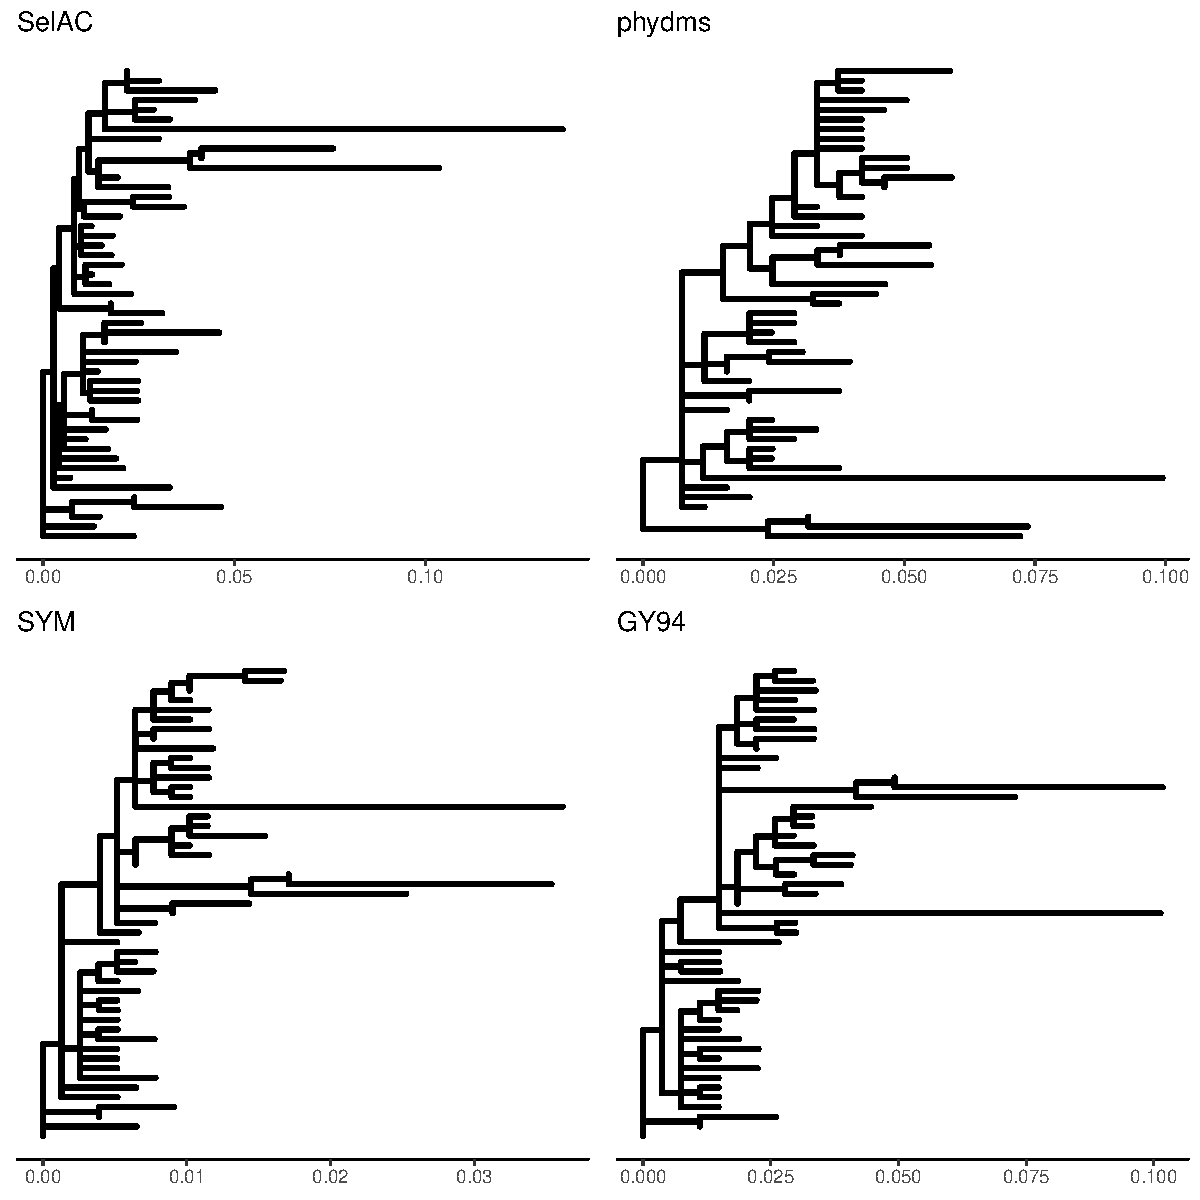
\includegraphics[width=\textwidth]{img/phy_TEM2016.pdf}
	\caption{Phylogenies estimated using \selac, \selac+DMS, \phydms, and \gy.}
	\label{fig:phylo}
\end{figure}





\subsection*{Laboratory inferences of selection are inconsistent with observed sequences.}
Improved model fits with phydms are deceiving.
The site specific selection inferred by the deep mutation scanning experiment is inconsistent with the observed TEM sequences.
We find that the sequence of selectively favored amino acids has only 49 \% sequence similarity with the observed consensus sequence (Figure \ref{fig:sim_seqs_cons}).
This is in contrast to the 99 \% of sequence similarity with the sequence of selectively favored amino acids estimated by \selac.

\begin{figure}[H]
     \centering
	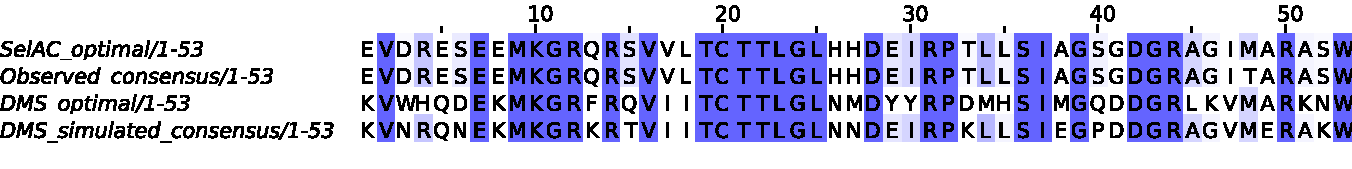
\includegraphics[width=\textwidth]{img/seq_simil_short.pdf}
	\caption{Every 5th residue. DMS and simulation based on DMS do not reflect natural sequences}
	\label{fig:sim_seqs_cons}
\end{figure}

Simulations of codon sequences under the experimentally inferred site specific selection for amino acids reveals that we would not expect to see the observed TEM sequences.
We simulated under a wide range of effective population sizes $N_e$, and find that the experimentally inferred site specific selection is very strong.
Only when $N_e$ is on the order of $10^0$ drift is overpowering the efficacy of selection.
With realistic values for $N_e = 10^7$, we find that the simulated sequences to show sequence similarity of $62 \%$ with the observed consensus sequence (Figure \ref{fig:dms_sim}a).
This is a higher similarity than the observed consensus sequence shows with the the sequence of selectively favored amino acids estimated using deep mutation scanning.
The genetic load of the simulated sequences deacrease slowely with increasing $N_e$ (Figure \ref{fig:dms_sim}b).
At time 1 and $N_e = 10^7$ the simulated sequences show a genetic load of 0.25, which is in contrast to the $\sim 8$ times higher observed load of 2.1.
Thus it appears unlikely that the observed sequences have evolved under the experimentally inferred site specific selection for amino acids.


\begin{figure}[h]
    \centering
    \begin{subfigure}
        \centering
        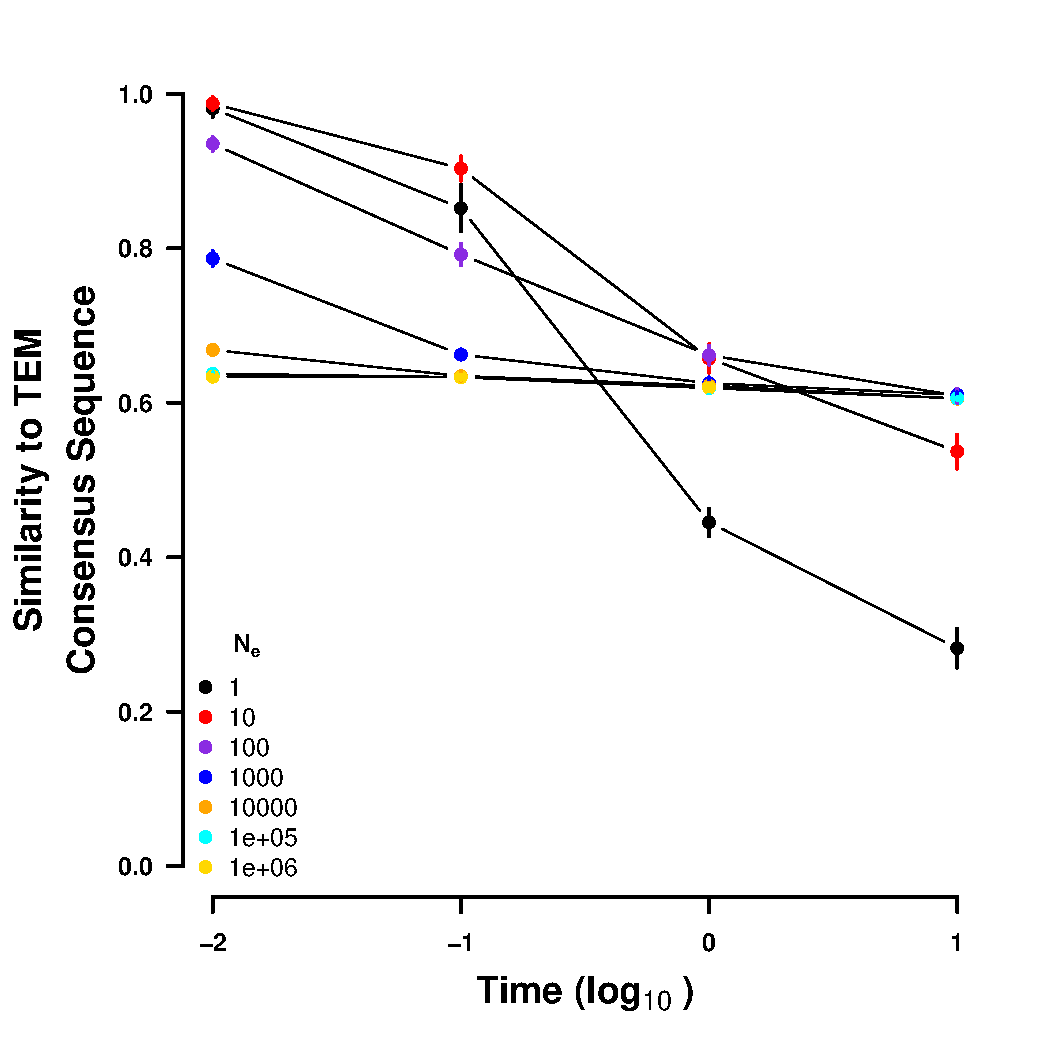
\includegraphics[width=.45\textwidth]{img/simulated_dist_time_DMS_ancest.pdf}
    \end{subfigure}
    \begin{subfigure}
        \centering
        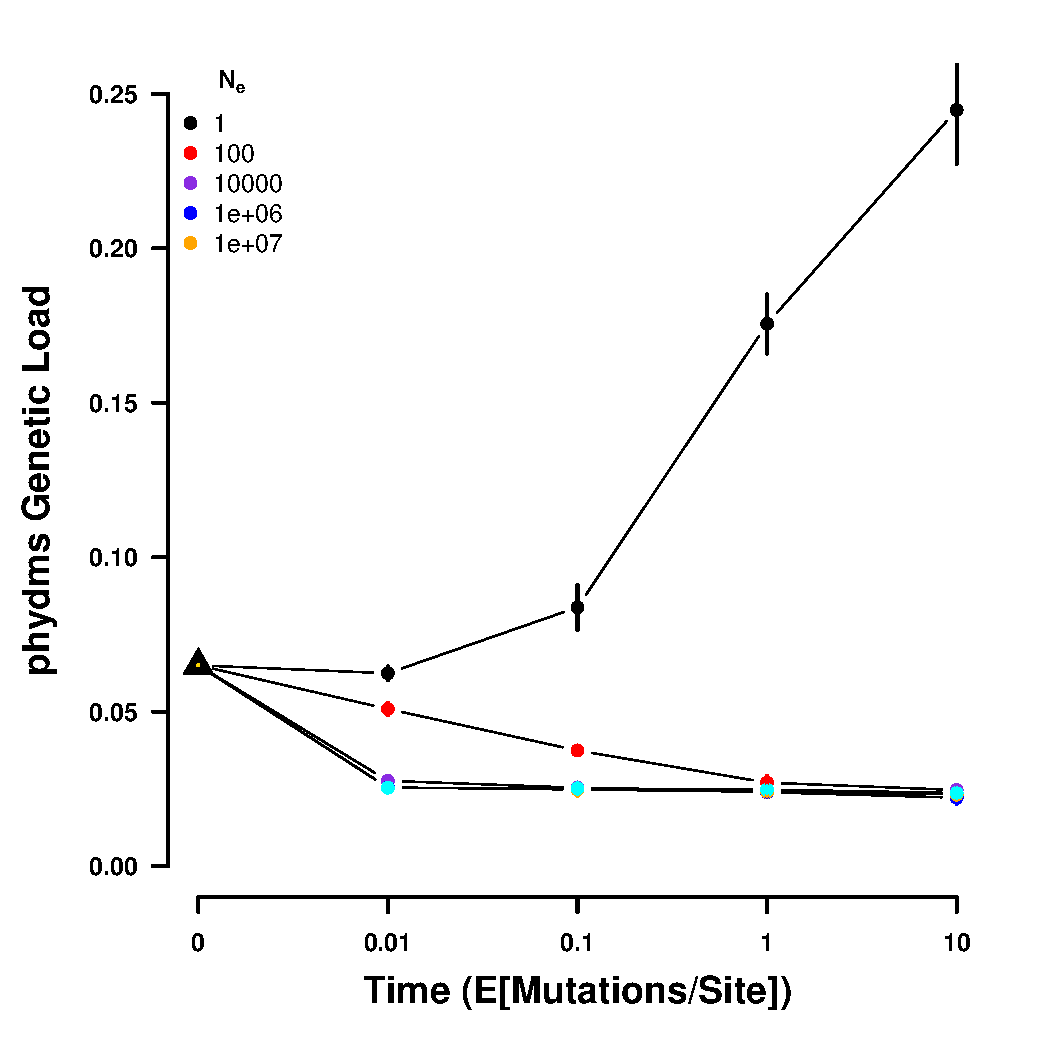
\includegraphics[width=.45\textwidth]{img/simulated_gl_time_DMS_ancest.pdf}
    \end{subfigure}
    \caption{Sequences simulated from the ancestral state under the site specific selection on amino acids estimated using deep mutation scanning. 
    (left) Sequence similarity to the observed consensus sequence at various times for a range on values of $N_e$.
    (right) Genetic load of the simulated sequences at various times for a range on values of $N_e$.
    Time is given in number of expected substitutions.
    Points indicate sample means and vertical bars indicate standard deviations. Initial sequence is the inferred ancestral state of the TEM variants and not shown.}
    \label{fig:dms_sim}
\end{figure}

\subsection*{\selac Model Adequacy} 
We assessed model adequacy and find that \selac better explains the observed TEM sequences.
The observed consensus sequence has a very high sequence similarity with the sequence of selectively favored amino acids estimated by \selac (99 \%).
Furthermore, assuming the site specific selection estimated by \selac, the observed sequences only show a minimal genetic load (Table \ref{tab:selection}, Figure \ref{fig:tem2016_sse}).

We simulated codon sequences forward in time for various length of time to assess the sequence similarity, assuming the \selac inferred site specific selection for amino acids.
% Ancestral starting point
We simulated the evolution of TEM from the inferred ancestral state using a wide range of effective population sizes $N_e$ (Figure \ref{fig:selac_sim}a).
The ancestral state state was estimated to be the observed consensus sequence.
For small $N_e$, we find that sequences drift away from the observed consensus. 
In turn, the genetic load increases drastically.
With increasing $N_e = 10^7$ the simulated sequences reach a sequence similarity at time 1 of $83 \%$, this is in contrast to the observed sequence similarity $98 \%$.
We calculated the genetic load at this time of the simulated sequences to be $9.8\times10^{-6}$ (Figure \ref{fig:selac_sim}b).
The genetic load of the observed sequences is estimated $4.2\times 10^{-5}$, one order of magnitute higher.
Thus, the simulated sequences show a lower genetic load despite the greater divergence from the observed consensus sequence.


\begin{figure}[h]
    \centering
    \begin{subfigure}
        \centering
        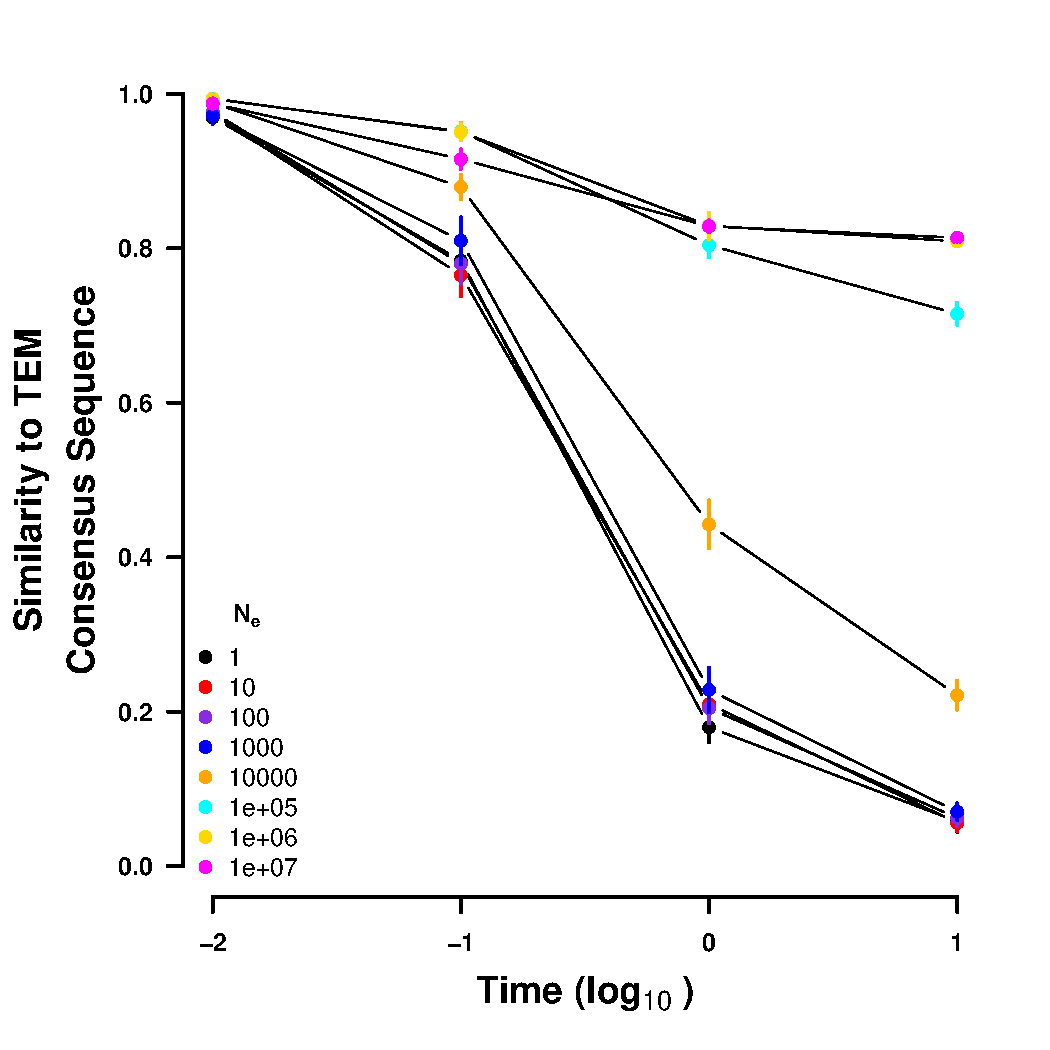
\includegraphics[width=.45\textwidth]{img/simulated_dist_time_SELAC_ancest.pdf}
    \end{subfigure}
    \begin{subfigure}
        \centering
        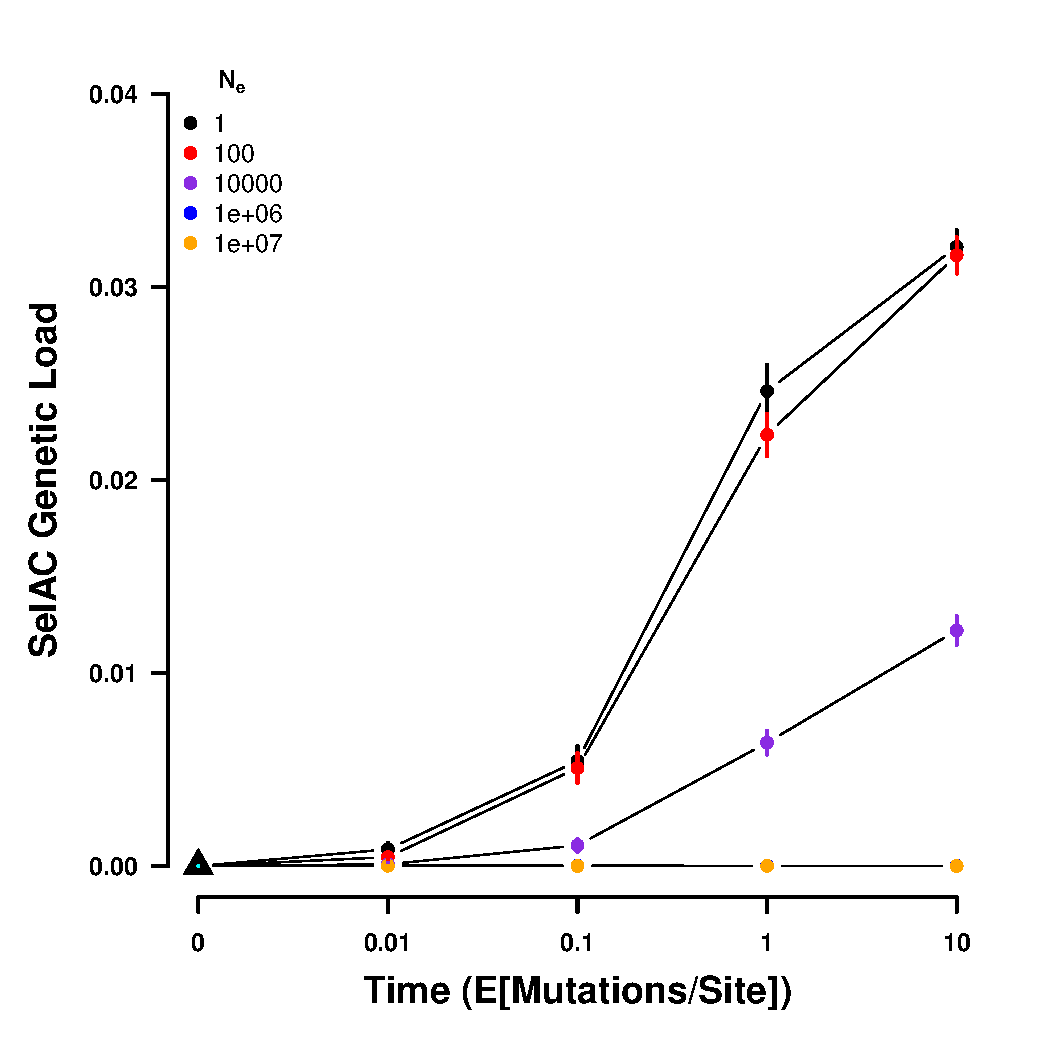
\includegraphics[width=.45\textwidth]{img/simulated_gl_time_SELAC_ancest.pdf}
    \end{subfigure}
    \caption{Sequences simulated from the ancestral state under the site specific selection on amino acids estimated using \selac. 
    (left) Sequence similarity to the observed consensus sequence at various times for a range on values of $N_e$.
    (right) Genetic load of the simulated sequences at various times for a range on values of $N_e$.
    Time is given in number of expected substitutions.
    Points indicate sample means and vertical bars indicate standard deviations. Initial sequence is the inferred ancestral state of the TEM variants and not shown.}
    \label{fig:selac_sim}
\end{figure}

% Random starting point
To further demonstrate the consistency of \selac, we utilized random codon sequences as starting points.
We find that the sequence similarity increases with effective population size $N_e$.
The random sequences start of with a similarity of $\sim6 \%$ which increases with $N_e$ to $\sim28 \%$ (Figure \ref{fig:selac_sim_rand}a).
The same initial sequences under the site specific selection inferred by the deep mutation scanning experiment increase only to $\sim18 \%$ in sequence similarity.



\subsection*{Site specific estimates of Selection on Amino Acids}
\selac allows for the site specific estimation of selection on amino acids and the genetic load of an observed amino acid relative to the inferred optimal amino acid.
We find that the genetic load is distributed along most of the observed TEM sequence with the exception of the region between residue 80 to 120 were three consequtive helices are located (Figure \ref{fig:tem2016_sse}). 
The most noticable increases in genetic load are found in unstructured regions
The largest increase in genetic load however, is located at the begining of the last helix.
We therefore estimate similar genetic loads for helices and unstructured regions in the observed TEM sequences (Table \ref{tab:selection})
The highest 
The Active sites appear to be under the strongest selection, with no accumulated genetic load.
This is in concordance with the experimental estimates.

\begin{table}
  \centering
  \begin{tabular}{llrrrr}
    Protein & Secondary Structure	& Mean G & SE G & Mean Genetic Load & SE Genetic Load \\ \hline 
    TEM	&		& 219.3 & 7.5 & $0.16\times10^{-7}$ & $6.5\times10^{-8}$ \\
    &Helix 		& 206.1 & 12.4 & $0.18\times10^{-7}$ & $0.13\times10^{-7}$ \\
    &Beta Sheet 	& 238.6 & 15.8 & $6.8\times10^{-8}$ & $2.9\times10^{-8}$ \\
    &Unstructured 	& 224.8 & 11.4 & $0.19\times10^{-7}$ & $8.1\times10^{-8}$ \\
    &Active Sites 	& 300   & 0    & 0      & 0      \\ \hline
    
    SHV&		& 244.9 & 6.8  & $4.0\times10^{-8}$ & $1.9\times10^{-8}$ \\
    &Helix		& 234.6 & 11.5 & $7.3\times10^{-8}$ & $4.8\times10^{-8}$ \\
    &Beta Sheet 	& 253.1 & 12.8 & $2.1\times10^{-8}$ & $1.1\times10^{-8}$ \\
    &Unstructured	& 250.3 & 11.0 & $1.8\times10^{-8}$ & $59\times10^{-8}$  \\
    &Active Sites	& 199.9 & 100  & $2.4\times10^{-8}$ & $2.4\times10^{-8}$ \\

  \end{tabular}
  \caption{Efficacy of selection (G) and Genetic Load for TEM and SHV and separated by secondary structure.}
  \label{tab:selection}
\end{table}

\begin{figure}[H]
     \centering
	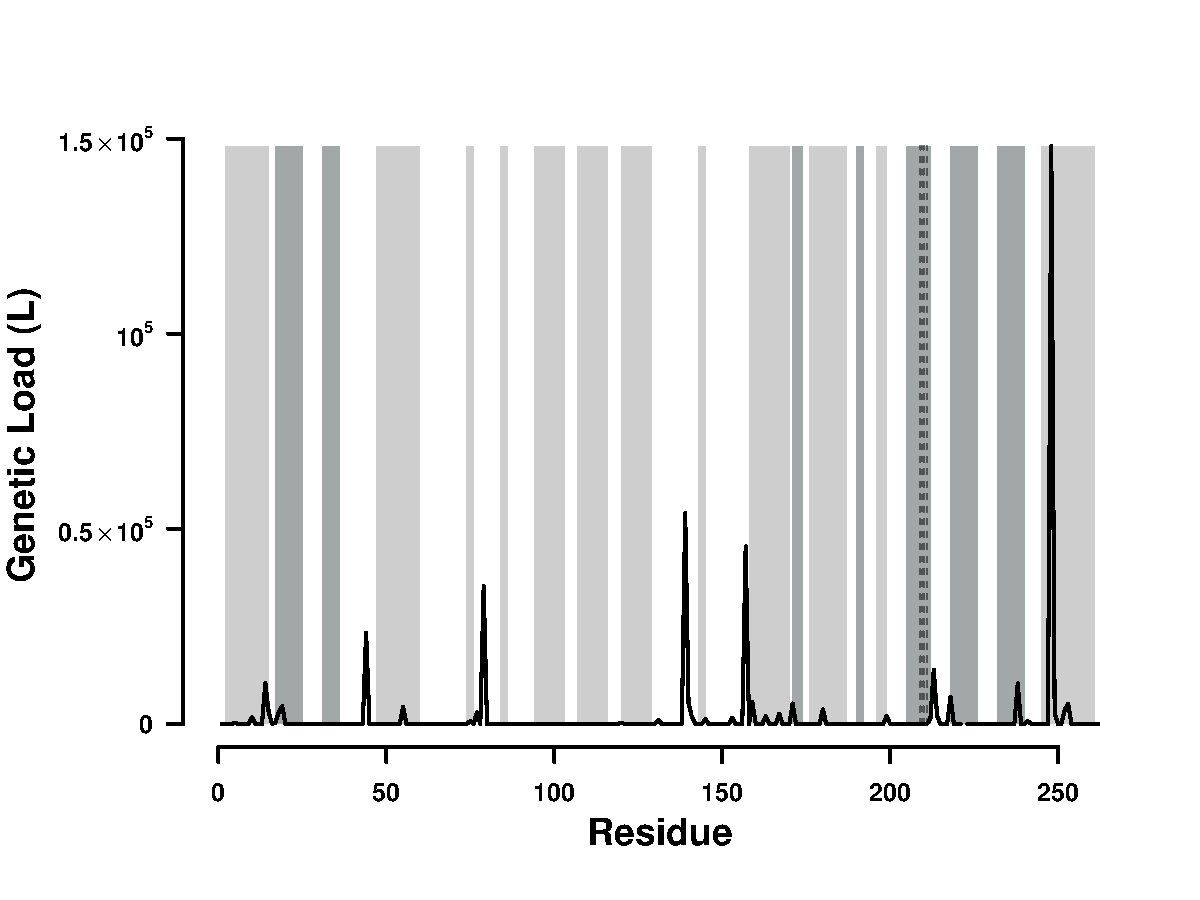
\includegraphics[width=\textwidth]{img/GL_slide_TEM2016}
	\caption{TEM, bars are different secondary structure elements. Dashed dotted line is DMS, solid is SelAC sNe, all lines are means of all sequences. vertical lines are active/binding sites.}
	\label{fig:tem2016_sse}
\end{figure}

It was previously proposed that experimentally inferred site specific selection for amino acids can be used to extraplotate the fitness landscape of related proteins \citep{bloom2014}.
We therefore compared the site specific efficacy of selection G, the \selac selection parameters of our \selac TEM model fit to a \selac model fit of SHV, and genetic load.
We find that site specific efficacy of selection G differes greatly between SHV and TEM ($\rho = 0.17$), despite a similar estimate of the parameter $\alpha_G$ describing the distribution of G values (Figure \ref{fig:tem_shv_param_comp}a).
With the expection of the active site, we find that G is increased in SHV (Table \ref{tab:selection}).
In general, most \selac selection parameters are very similar between the TEM and the SHV model fit. 
An exception is the weight for the physicochemical composition property $\alpha_c$ (Figure \ref{fig:tem_shv_param_comp}b).

The genetic load in SHV is by an order of magnitute lower than in TEM with the exception of residues found in $\beta$-sheets and the active site (Table \ref{tab:selection}).
This is consitent with the elevated site specific efficacy of selection G in SHV.
As a comparison of site specific efficacy of selection G already indicated, the sites introducing genetic load differ between SHV and TEM (Figure \ref{fig:shv2016_sse}).
We find the highest genetic load in SHV at the end of the first helix.
However, we do find a peak of similar magnitute in the TEM sequence at the end of the first helix.


\section*{Discussion}

We evaluated how well experimental selection estimates from laboratory experiments, specifically deep mutation scanning, explain sequence evolution and compared it to \selac, a novel phylogenetic framework.
Previous work has shown that laboratory estimates of selection can improve model fit over classical approaches like GY94 \citep{bloom2014, bloom2017}.
While our study confirms this notion, we also raise awarness for shortcomings of these laboratory estimates and propose a more general applicable alternative.
\selac, in contrast, is a more general alternative that does not depend on costly laboratory estimates of selection and is favored by model selectin (Table \ref{tab:AIC}).

While previous work showed the advantages of experimentally informed phylogenetics estimates, they did not assess how adequate the estimated selection reflects observed sequences.
This becomes abherent in the low sequence similarity between the observed consensus sequence and the sequence of selectively favored amino acids estimated from deep mutation scanning experiments.
In contrast, the selectively favored amino acids estimated by \selac shows a high sequence similarity with the observed consensus sequence.
This begs the question how well the experimental selection coefficients represent evolution.
Deep mutation scanning experiments are performed using a comprehensive library of mutants and a strong artificial selection pressure \citep{FirnbergAndOstermeier2012, Jain2014, FowlerAndFields2014, Fowler2014}.
This results in a very large selection coefficient $s$ and a competing heterogeneous population.

The induced selection pressure during the deep mutation scanning experiment was limited to ampicillin \citep{stiffler2016} and focused on the TEM-1 variant.
However, TEM can also confer resistance to a wide range of other antibiotics, like other penicillins, cephalosporins, cefotaxime, ceftazidime, or aztreonam.
Thus, the inferred selection is biased towards ampicillin and is therefore unlikely to reflect the evolution the observed TEM variants have experienced.
We therfore propose to include a variety of selection pressures if the experimental selection estimates are used for phylogenetic inference.

TODO:  Lack of repeatability between labs introduces further problems (Firnberg et al 2014 vs. Stifler et al. 2016).




\begin{itemize}
	\item We evaluated how well experimental selection estimates from DMS experiments explain natural sequence evolution and compared it to a novel phylogenetic framework, SelAC.
	\begin{itemize}
		\item Previous work has shown that DMS selection estimates can improve model fit over classical approaches like GY94 and our work confirms this.
		\item Model selection favored the SelAC model fit and the corresponding fitness estimates over the DMS estimates using both, SelAC and phyDMS (Table \ref{tab:AIC}).
	\end{itemize}

	\item Adequacy of the DMS selection has previously not been assessed.
	\begin{itemize}
		\item The amino acid with the cumulative highest fitness experimentally estimated with DMS only has $49 \%$ concordance with the observed alignment.
		\item In contrast, the SelAC estimate has $99 \%$ concordance (Figure \ref{fig:sim_seqs_cons}). 
		\item Estimates of selection coefficients do not represent evolution.
 		\begin{itemize}
			\item Due to artificial selection environment; Heterogeneous population, very large $s$. 
			\item Only one antibiotic used, maybe a mixture of antibiotics would better reflect natural evolution.
			\item Lack of repeatability between labs introduces further problems (Firnberg et al 2014 vs. Stifler et al. 2016).
		\end{itemize}
	\end{itemize}

	\item Assuming that the DMS selection inference adequately reflects natural evolution, the observed TEM sequences are either mal-adapted or where unable to reach a fitness peak.
	\begin{itemize}
		\item \textit{E. coli} has a large effective population size, estimates are on the order of $10^8$ to $10^9$ (Ochman and Wilson 1987, Hartl et al 1994).
		\item The large $N_e$ would allow \textit{E. coli} to effectively "explore" the sequence space, thus suggesting that the TEM sequences are mal-adapted according to the DMS estimates.
		\item Our simulations of sequence evolution with various $N_e$ values and the DMS fitness values in contrast show that we would expect higher adaptation even with much smaller $N_e$ (Figure \ref{fig:dms_sim}).
	\end{itemize}

	\item Estimates of selection coefficients do not represent evolution.
 	\begin{itemize}
		\item Due to artificial selection environment; Heterogeneous population, very large $s$. 
		\item Only one antibiotic used, maybe a mixture of antibiotics would better reflect natural evolution.
		\item Lack of repeatability between labs introduces further problems (Firnberg et al 2014 vs. Stifler et al. 2016).
		\item Still better than models without site specific equilibrium frequencies.
	\end{itemize}

	\item DMS estimates of the observed TEM variants predict them to be mal-adapted while SelAC predicts most TEM variants to be well adapted.
	\begin{itemize}
		\item Given \textit{E. coli}'s large effective population size, the efficacy of selection should be very large.
		\item We therefore expect the observed sequence variants to be at the selection-mutation-drift barrier, which in turn can expected to be near the optimum.
		\item We find the majority of sequences near the optimum, therefore the SelAC estimates are consistent with theoretical population genetics results.
		\item In contrast, finding strong selection against the observed TEM variants indicates that DMS is not consistent with theoretical population genetics expectations.
		\item This is consistent when thinking about that DMS only reflects the selection on the TEM sequence with regards to one antibiotic, which seems appropriate to model selection in modern hospital environments but not when the interest lies in the natural evolution of TEM.
	\end{itemize}

	\item We find that SelAC produces similar selection against the observed TEM variants  if we assume the fitness peaks (optimal AA) that are estimated by DMS.
	\begin{itemize}
		\item This shows that DMS and SelAC can provide consistent estimates of selection against amino acids.
		\item SelAC has the advantage that it can be applied to any protein coding sequence alignment.
		\item This removes the need for extrapolation e.g. from TEM to SHV.
	\end{itemize}

	\item SelAC has the advantage that it can be applied to any protein coding sequence alignment.
	\begin{itemize}
		\item This removes the need for extrapolation e.g. from TEM to SHV.
	\end{itemize}

	\item Difference in selection parameters between TEM and SHV indicate that extrapolation is not a good idea.
	\begin{itemize}
		\item The difference in the site specific strength of selection shows that TEM and SHV are facing different selection pressures.
		\item this is also highlighted by the differences in physicochemical weightings between the two proteins.
	\end{itemize}

	\item SelAC outperforms DMS, but is not without flaws itself
	\begin{itemize}
		\item Like DMS and most phylogenetic models, SelAC assumes site independence.
		\item SelAC is a model of stabilizing selection, in contrast to e.g. GY94 which is a model of frequency dependent selection.
		\begin{itemize}
			\item Since TEM plays a role in the chemical warfare with conspecifics and other microbes, some sites may be under negative frequency dependent selection.
		\end{itemize}
		\item SelAC assumes the same G distribution across all sites.
		\begin{itemize}
			\item Different G distribution for each type of secondary structure
			\item active sites may not follow distribution.
		\end{itemize}
		\item SelAC assumes that selection is proportional to distance in physicochemical space. 
		\begin{itemize}
			\item We used Grantham (1974) properties, however many other distances are available which may an even better model fit.
		\end{itemize}
	\end{itemize}
	\item Low sequence variation in the TEM may be cause for concern as it could be misinterpreted by the model as stabilizing selection because of the short branches.
	\begin{itemize}
		\item However, provided our simulations support that TEM is actually under stabilizing selection
	\end{itemize}

	\item In conclusion, DMS experiments have been proposed to supplement information on selection on amino acids in phylogenetic studies.
	\begin{itemize}
		\item This study shows that information on selection can be extracted from alignments of protein coding sequences.
		\item This highlights the limitations of DMS to explain natural evolution.
	\end{itemize}
\end{itemize}


\section*{Materials and Methods}

\subsection*{Phylogenetic Inference and Model selection}

TEM and SHV sequences were obtained from \citet{bloom2017} already aligned.
We however, separated the TEM and SHV sequences into individual alignemnts.
Experimentally fitness values for TEM were taken from \citet{stiffler2016}.
We followed \citep{bloom2017} to convert the experimental fitness values into site specific equilibrium frequencies for \phydms. 

\selac (version 1.6.1) was fitted to the TEM alignment using R (version 3.4.1) \citep{rcore} with and without site specific selection on amino acids estimated from deep mutation scanning experiments.
\phydms (version 2.5.1) was fitted using site specific selection on amino acids estimated from deep mutation scanning experiments from \citet{stiffler2016} and python (version 3.6).
All other models were fitted using IQTree \citep{nguyen2015}.

We report each model's $\log(\Lik)$, AIC, and  AICc. 
Models were selected based on the AICc values.

\subsection*{Sequence Simulation}

Sequences were simulated by stochastic simulations using a Gillespie algorithm \citep{gillespie1976} that was model independent.
The simulation followed \citet{SellaAndHirsh2005} to calculate fixation probabilities.
The fitness values were estimated using \selac or experimentally inferred.
We chose the fitnest values of the highest concentration (2500 $\mu g/mL$) treatment of ampicillin for our comparison.
We modified the experimental fitness such that the amino acid with the highest fitness at each site has a value of one.
Mutation rates were taken from the \selac or \selac+DMS fit.
The initial sequences were either a random sample of 263 codons or the ancestral sequence reconstructed using FastML \citep{fastml} (last accessed: 30.09.2018).
Each sequence was simulated 10 times and we report average genetic load and sequence similarity and the corresponding standard error.

\subsection*{Estimating site specific G}


\subsection*{Estimating site specific fitness values $w_i$}

Following \citet{beaulieu2018} $w_i$ is proportional to
\begin{equation}
w_i \propto \exp(-A_0\eta\psi)
\end{equation}
were $A_0$ decribes the decline in fitness with each high energy phosphate bond, and $\psi$ is the protein's production rate.
$\eta$ is the cost/benefit ratio of a protein (see \citep{beaulieu2018} for details). 
However, \selac only estimates a composition parameter $\psi' = A_0\times\psi\times N_e\times q$.
$N_e$ describes the effective population size and is assumed by \selac to be $5\times 10^6$.
$q$ is the XXX and is assumed by \selac to be $4\times 10^{-7}$.
$A_0$ assumed to be $4$.
Thus, 
\begin{equation}
\psi = \frac{\psi'}{A_0N_eq}
\end{equation}


\subsection*{Model Adequacy}

Model adequacy was assessed by comparing the observed sequences and simulations under the site specific selection inferred by the deep mutation scanning experiment or \selac.
First, similarity between the sequence of selectively favored amino acids and the observed TEM sequences was assessed.
Sequence similarity was measured as the number of differences in the amino acid sequence.
Second, the genetic load of the observed and the simulated sequences was calculated using either the site specific selection inferred by the deep mutation scanning experiment or \selac.

Genetic load was calculated as
\begin{equation}
L_i = \frac{w_{max} - w_i}{w_{max}}
\end{equation}
were $w_{max}$ is the fitness of the sequence of selectively favored amino acids estimated using  the site specific selection inferred by the deep mutation scanning experiment or \selac.
$w_i$ represents the fitness of the $i$th residue.
This the genetic load $L$ of a sequence is given by $\sum_{i=1}^n L_i$ where $n$ is the number of amino acids.



\bibliographystyle{unsrtnat}
\bibliography{ecoli}

\section*{Figures}



\beginsupplement
\section*{Supplementary Figures}


\begin{figure}[H]
     \centering
	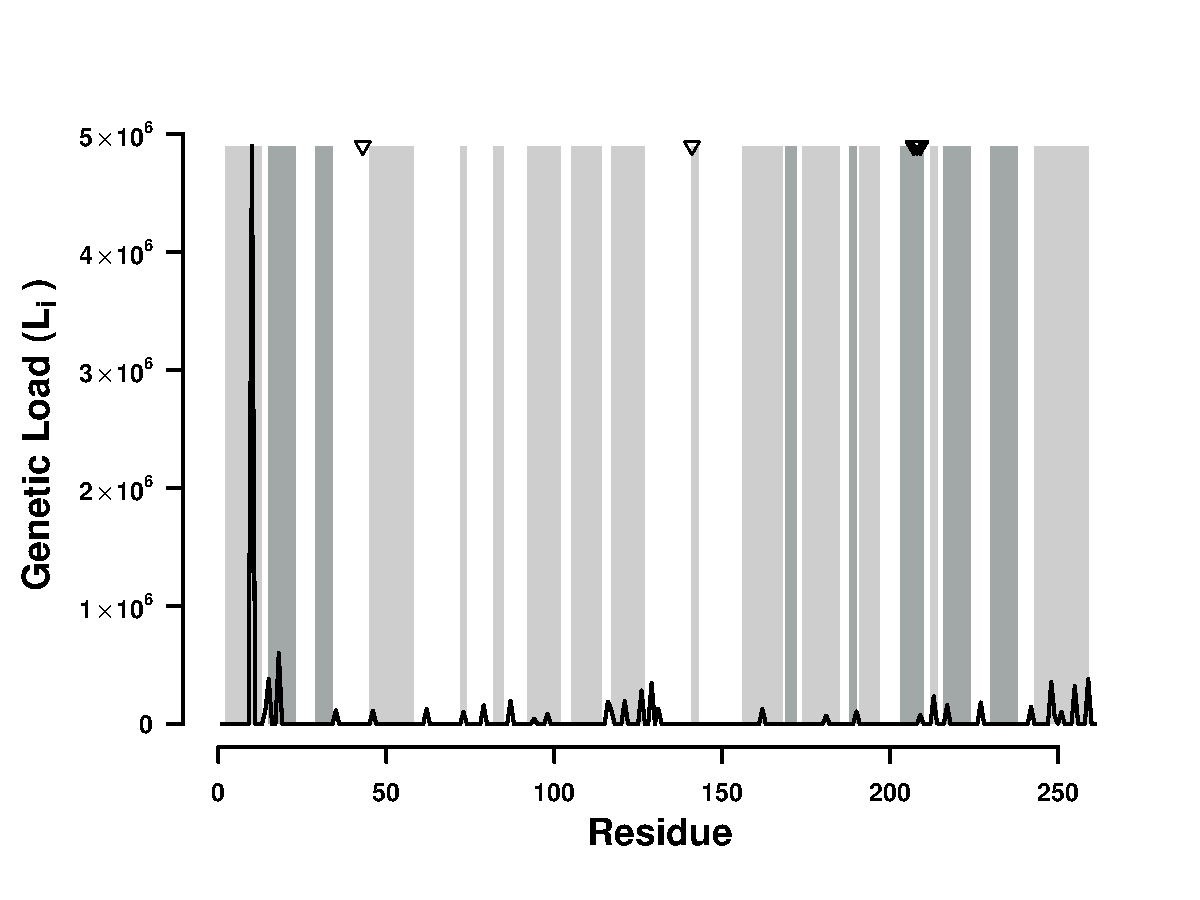
\includegraphics[width=\textwidth]{img/GL_slide_SHV2016}
	\caption{SHV, bars are different secondary structure elements. Dashed dotted line is DMS, solid is SelAC sNe, all lines are means of all sequences. vertical lines are active/binding sites.}
	\label{fig:shv2016_sse}
\end{figure}

\begin{figure}[h]
    \centering
    \begin{subfigure}
        \centering
        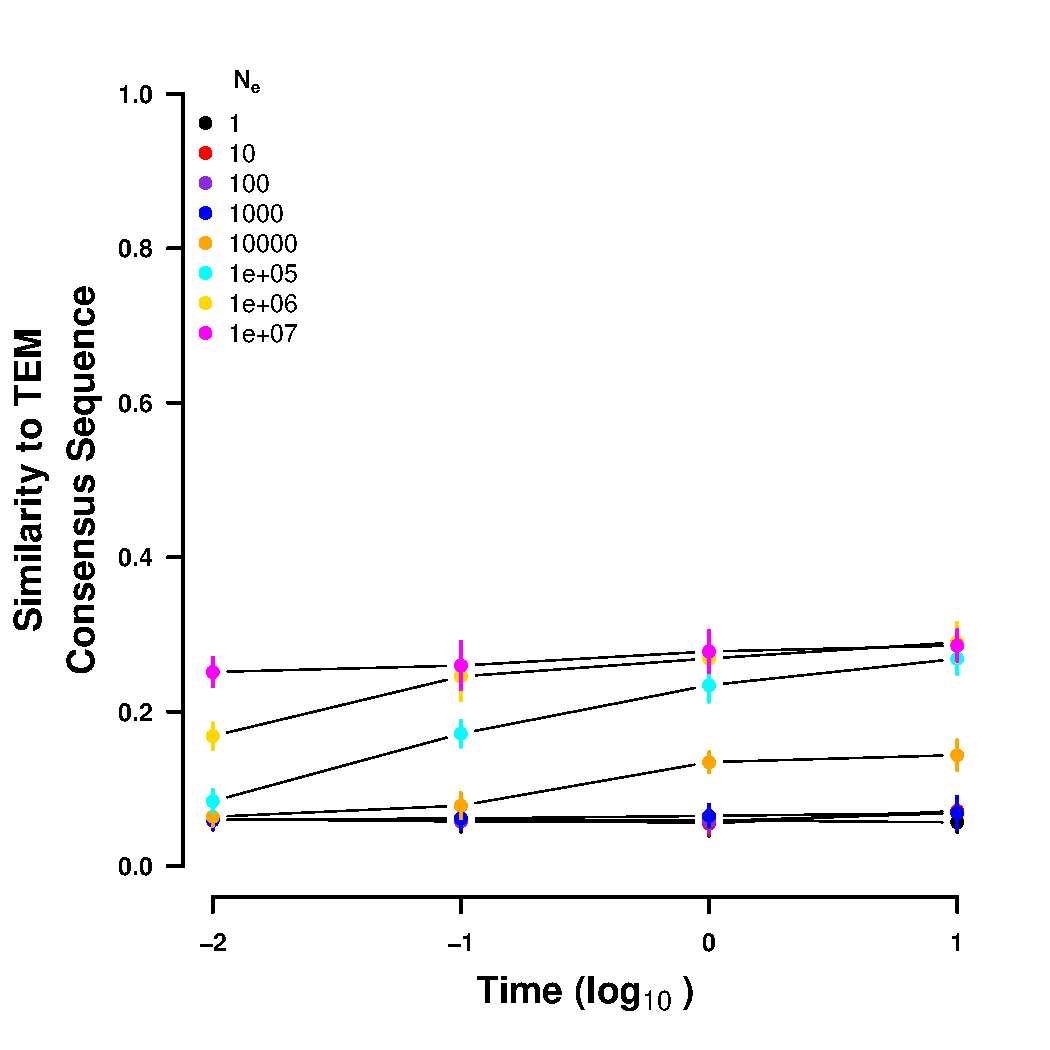
\includegraphics[width=.45\textwidth]{img/simulated_dist_time_SELAC_random.pdf}
    \end{subfigure}
    \begin{subfigure}
        \centering
        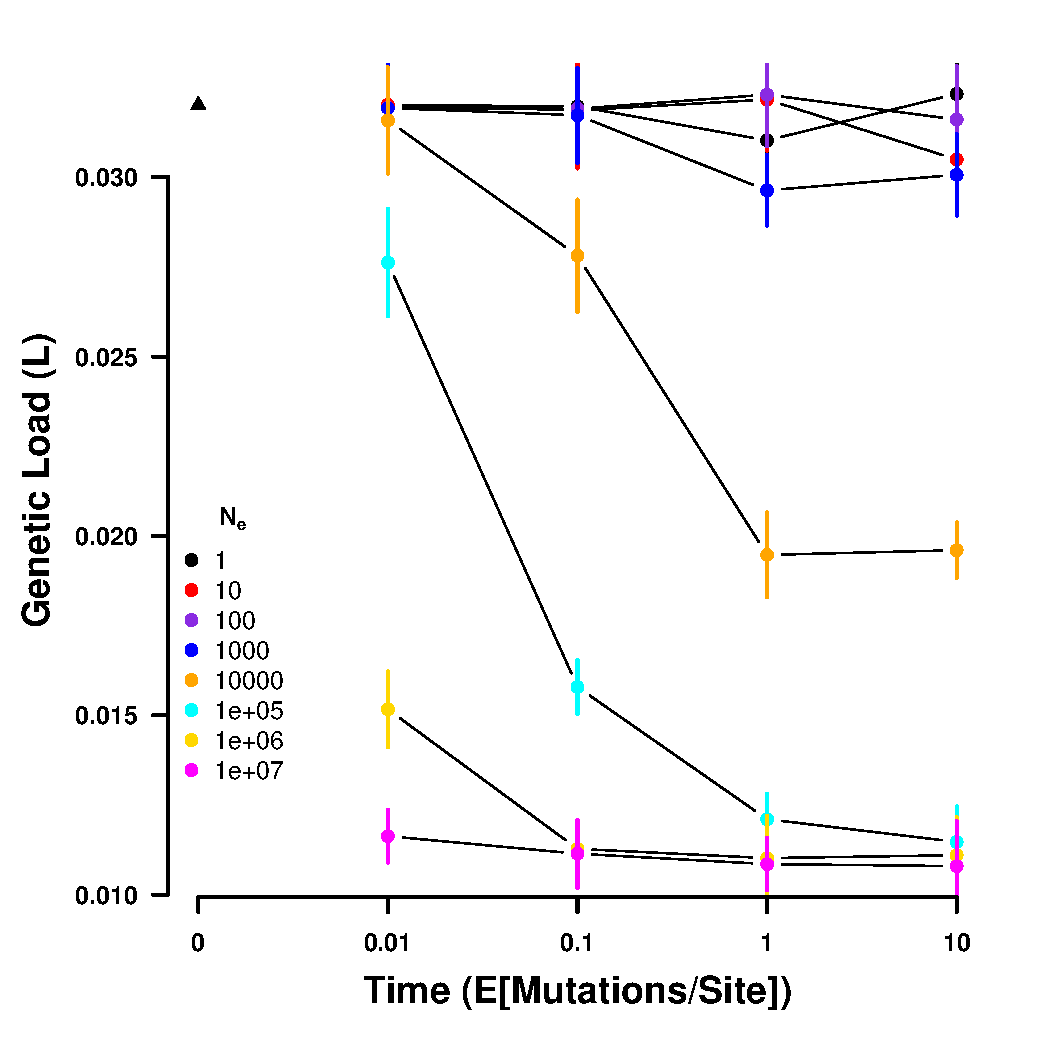
\includegraphics[width=.45\textwidth]{img/simulated_gl_time_SELAC_random.pdf}
    \end{subfigure}
    \caption{{Sequences simulated from a random codon sequence under the site specific selection on amino acids estimated using \selac. 
    (left) Sequence similarity to the observed consensus sequence at various times for a range on values of $N_e$.
    (right) Genetic load of the simulated sequences at various times for a range on values of $N_e$.
    Time is given in number of expected substitutions.
    Points indicate sample means and vertical bars indicate standard deviations. Initial sequence is the inferred ancestral state of the TEM variants and not shown.}}
    \label{fig:selac_sim_rand}
\end{figure}

\begin{figure}[h]
    \centering
    \begin{subfigure}
        \centering
        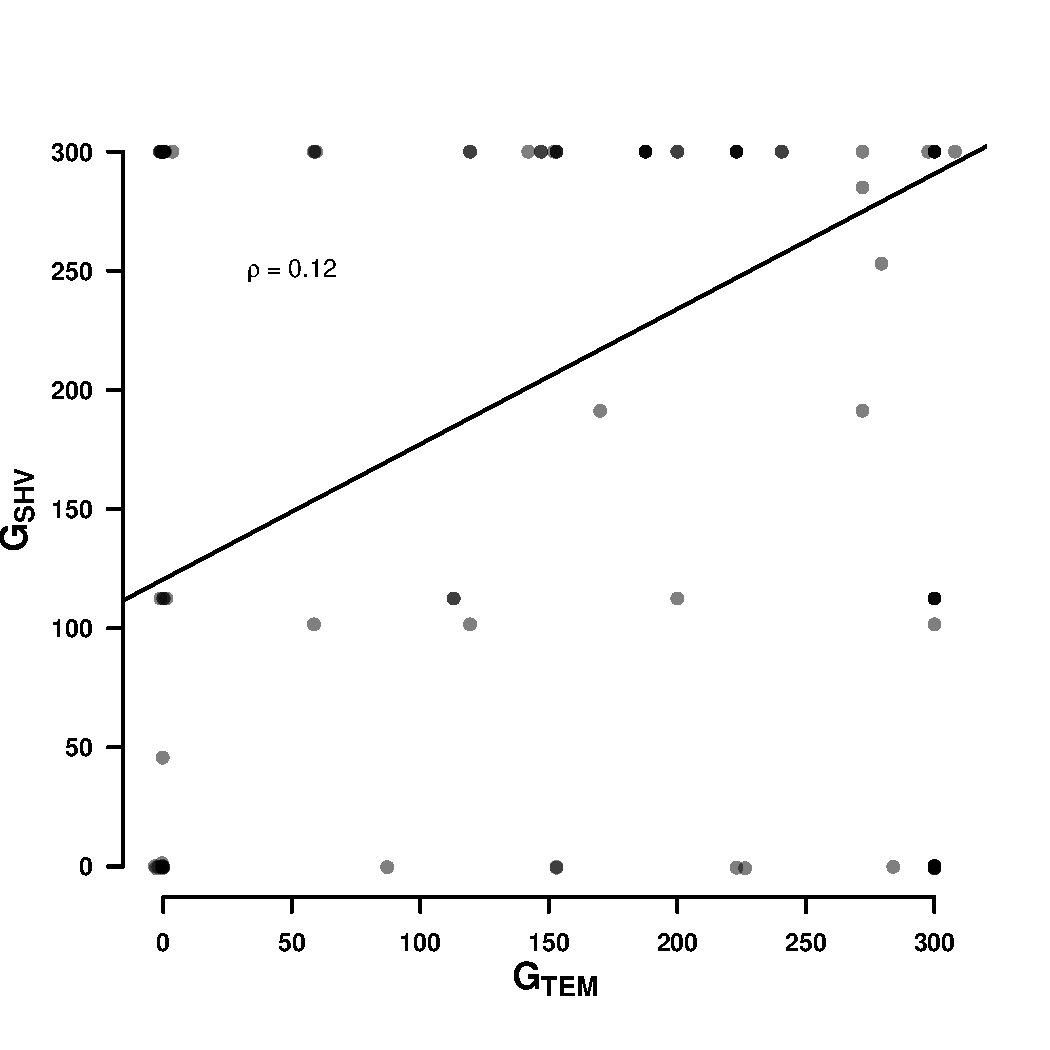
\includegraphics[width=.45\textwidth]{img/g_shift_lac.pdf}
    \end{subfigure}
    \begin{subfigure}
        \centering
        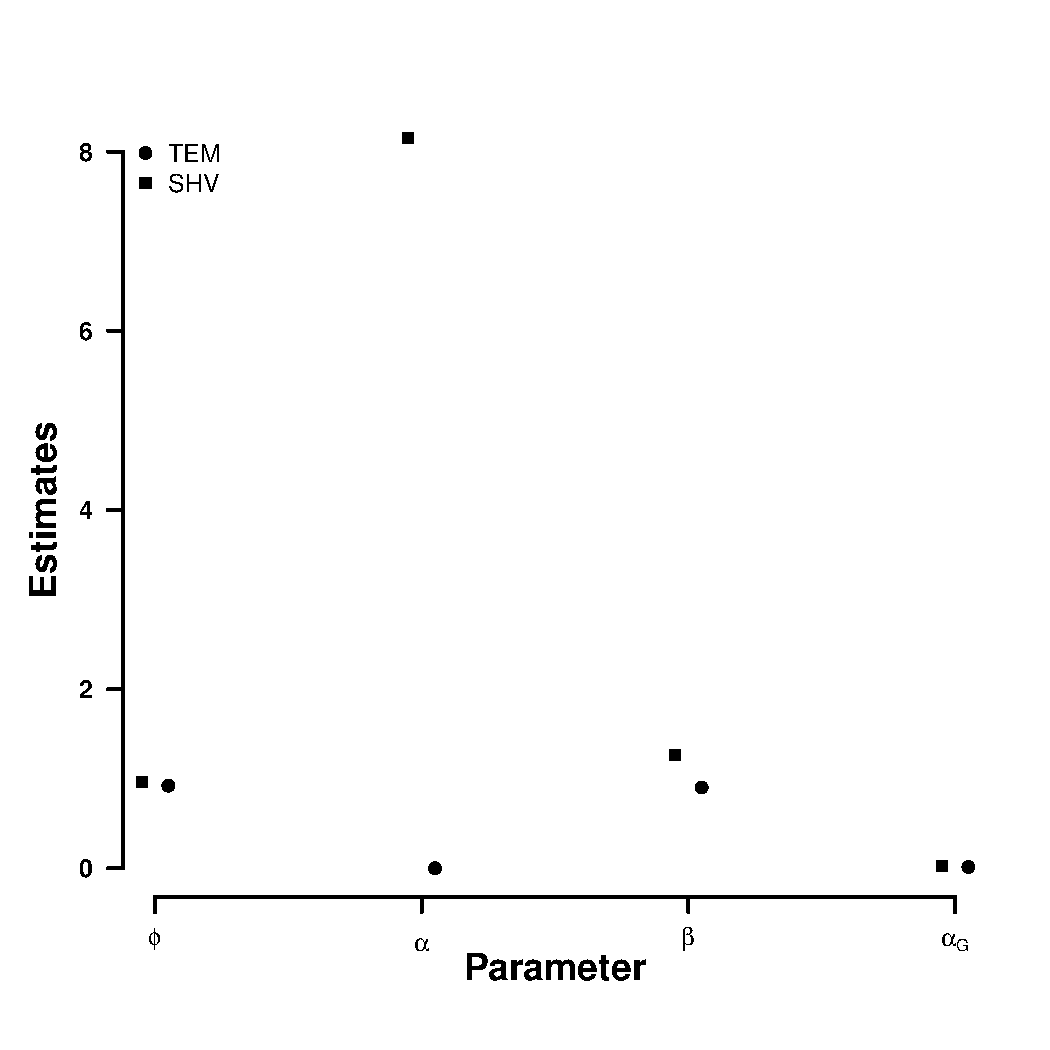
\includegraphics[width=.45\textwidth]{img/TEM_SHV_2016_par_comp.pdf}
    \end{subfigure}
    \caption{Comparisson of selection related parameters between TEM and SHV.}
    \label{fig:tem_shv_param_comp}
\end{figure}

\end{document}
